% -----------------------------------
% -----------------------------------
% abnTeX2: Normas ABNT NBR 14724:2011 + sugestões FGV/EMAp. 

% Autor: Lauro César Araujo
% Adaptações EMAp: Lucas Machado Moschen 
% Copyright 2012-2018 by abnTeX2 group at http://www.abntex.net.br/ 

%% This work may be distributed and/or modified under the
%% conditions of the LaTeX Project Public License, either version 1.3
%% of this license or (at your option) any later version.
%% The latest version of this license is in
%%   http://www.latex-project.org/lppl.txt
%% and version 1.3 or later is part of all distributions of LaTeX
%% version 2005/12/01 or later.
% ----------------------------------
% ----------------------------------
\documentclass[
	% -- opções da classe memoir --
	12pt,				% tamanho da fonte
	%openright,			% capítulos começam em página ímpar (insere página vazia caso preciso)
	oneside,			% para impressão em recto e verso. Oposto a oneside
	a4paper,			% tamanho do papel. 
	% -- opções da classe abntex2 --
	%chapter=TITLE,		% títulos de capítulos convertidos em letras maiúsculas
	%section=TITLE,		% títulos de seções convertidos em letras maiúsculas
	%subsection=TITLE,	% títulos de subseções convertidos em letras maiúsculas
	%subsubsection=TITLE,% títulos de subsubseções convertidos em letras maiúsculas
	% -- opções do pacote babel --
	english,			% idioma para inglês
	brazil				% idioma para português
	]{abntex2}

%------------------------------------------------
%-------------- Pacotes necessários -------------
%------------------------------------------------

% Escrita 
\usepackage[T1]{fontenc}
\usepackage[utf8]{inputenc}
\usepackage{lmodern}
\usepackage{microtype} % para melhorias de justificação
\usepackage{indentfirst}

\renewcommand{\ABNTEXchapterfont}{\fontfamily{ptm}\fontseries{b}\selectfont}

% Gráficos 
\usepackage{color}
\usepackage{caption}
\usepackage{subcaption}
\usepackage{graphicx}
\graphicspath{{../../images/}}

% Matemáticos 
\usepackage{amsthm, amssymb, amsmath, mathtools}

% Outros 
\usepackage{lipsum}


% Citações 
%\usepackage[brazilian,hyperpageref]{backref}
%\usepackage[alf]{abntex2cite}	% Citações padrão ABNT
\usepackage[style=abnt]{biblatex}
\addbibresource{biblio.bib}  

% \renewcommand{\backrefpagesname}{Citado na(s) página(s):~}
% % Texto padrão antes do número das páginas
% \renewcommand{\backref}{}
% % Define os textos da citação
% \renewcommand*{\backrefalt}[4]{
% 	\ifcase #1 %
% 		Nenhuma citação no texto.%
% 	\or
% 		Citado na página #2.%
% 	\else
% 		Citado #1 vezes nas páginas #2.%
% 	\fi}%
% ---

%----------------------------------------
%------- Capa e Folha de Rosto ----------
%----------------------------------------

\newcommand\subtitulo[1]{\def\@subtitulo{#1}}
\newcommand{\imprimirsubtitulo}{\@subtitulo}

\renewcommand{\imprimircapa}{%
	\begin{capa}%
	\center
		\ABNTEXchapterfont\Large \MakeUppercase{\imprimirinstituicao}
		\\\vspace*{4cm}
		{\ABNTEXchapterfont\large \MakeUppercase{\imprimirautor}}
		\vfill
		\begin{center}
		\ABNTEXchapterfont\large\MakeUppercase{\imprimirtitulo}
		\end{center}
		\vfill
		\normalfont\large\imprimirlocal
		\\\normalfont\large\imprimirdata
		\vspace*{1cm}
	\end{capa}
}

\makeatletter
\renewcommand{\folhaderostocontent}{
  \begin{center}

    %\vspace*{1cm}
    {\ABNTEXchapterfont\large\MakeUppercase{\imprimirautor}}
	
    \vspace*{\fill}\vspace*{\fill}
    \begin{center}
      \ABNTEXchapterfont\bfseries\large\MakeUppercase{\imprimirtitulo}
    \end{center}
    \vspace*{\fill}
	
    \abntex@ifnotempty{\imprimirpreambulo}{%
      \hspace{7.5cm}
      \begin{minipage}{.5\textwidth}
      	\SingleSpacing
         \imprimirpreambulo
         \\\\
         Orientador: \imprimirorientador
       \end{minipage}%
       \vspace*{\fill}
    }%

    % {\large\imprimirorientadorRotulo~\imprimirorientador\par}
    % \abntex@ifnotempty{\imprimircoorientador}{%
    %    {\large\imprimircoorientadorRotulo~\imprimircoorientador}%
    % }%
    \vspace*{\fill}

    {\large\imprimirlocal}
    \par
    {\large\imprimirdata}
    \vspace*{1cm}

  \end{center}
}
\makeatother

\titulo{Síntese de Texturas Baseado em Amostra}
\autor{Danilo Lemos Cardoso}
\local{Rio de Janeiro}
\data{2022}
\instituicao{%
  Fundação Getulio Vargas \\
  \par
  Escola de Matemática Aplicada
}
\tipotrabalho{Trabalho de Conclusão de Curso}

\preambulo{Trabalho de conclusão de curso apresentada para a Escola de
Matemática Aplicada (FGV/EMAp) como requisito para o grau de bacharel em
Matemática Aplicada. \\ \\ Área de estudo: area de estudo.}

\orientador{Asla Medeiros e Sá}

% Se o seu texto tem subtítulo. 
% Se não tiver, altere o arquivo capa_folha_rosto_tex
%\subtitulo{POKEMON}

%---------------------------------------------
%-------------------- PDF --------------------
%---------------------------------------------

% alterando o aspecto da cor azul
\definecolor{blue}{RGB}{41,5,195}

% informações do PDF
\makeatletter
\hypersetup{
     	%pagebackref=true,
		pdftitle={\@title}, 
		pdfauthor={\@author},
    	pdfsubject={\imprimirpreambulo},
	    pdfcreator={LaTeX with abnTeX2},
		pdfkeywords={abnt}{latex}{abntex}{abntex2}{trabalho acadêmico}, 
		colorlinks=true,       		% false: boxed links; true: colored links
    	linkcolor=blue,          	% color of internal links
    	citecolor=blue,        		% color of links to bibliography
    	filecolor=magenta,      		% color of file links
		urlcolor=blue,
		bookmarksdepth=4
}
\makeatother

% Posiciona figuras e tabelas no topo da página quando adicionadas sozinhas
% em um página em branco. Ver https://github.com/abntex/abntex2/issues/170
\makeatletter
\setlength{\@fptop}{5pt} % Set distance from top of page to first float
\makeatother

%---------------------------------------
%--------- Mais configurações-----------
%---------------------------------------

% Possibilita criação de Quadros e Lista de quadros.
% Ver https://github.com/abntex/abntex2/issues/176
\newcommand{\quadroname}{Quadro}
\newcommand{\listofquadrosname}{Lista de quadros}

\newfloat[chapter]{quadro}{loq}{\quadroname}
\newlistof{listofquadros}{loq}{\listofquadrosname}
\newlistentry{quadro}{loq}{0}

% configurações para atender às regras da ABNT
\setfloatadjustment{quadro}{\centering}
\counterwithout{quadro}{chapter}
\renewcommand{\cftquadroname}{\quadroname\space} 
\renewcommand*{\cftquadroaftersnum}{\hfill--\hfill}

\setfloatlocations{quadro}{hbtp} % Ver https://github.com/abntex/abntex2/issues/176

%-----------------------------------------------------
%--------------------- Margens -----------------------
%-----------------------------------------------------

\setlrmarginsandblock{3cm}{2cm}{*}
\setulmarginsandblock{3cm}{2cm}{*}
\checkandfixthelayout

%-----------------------------------------------------
%------ Espaçamentos entre linhas e parágrafos -------
%-----------------------------------------------------

% O tamanho do parágrafo é dado por:
\setlength{\parindent}{1.3cm}

% Controle do espaçamento entre um parágrafo e outro:
\setlength{\parskip}{0.2cm}  % tente também \onelineskip

% compila o índice
\makeindex

%------------------------------------------------------
%----------- Personal Definitions ---------------------
%------------------------------------------------------

\newcommand{\R}{\mathbb{R}}
\newcommand{\x}{\boldsymbol{x}}
\newcommand{\N}{\operatorname{Normal}}
\newcommand{\betadist}{\operatorname{Beta}}
\newcommand{\bern}{\operatorname{Bernoulli}}
\newcommand{\tril}{\operatorname{tril}}

\newcommand{\ev}{\mathbb{E}}
\newcommand{\var}{\operatorname{Var}}
\newcommand{\cor}{\operatorname{Cor}}
\newcommand{\cov}{\operatorname{Cov}}

\newtheorem{theorem}{Theorem}[]
\newtheorem{proposition}{Proposition}[]

\theoremstyle{definition}
\newtheorem{definition}{Definition}[section]

\theoremstyle{remark}
\newtheorem*{remark}{Remark}
\newtheorem{assumption}{Assumption}

\newcommand{\improve}[1]{\textcolor{red}{#1}}

%-------------------------------------------------
%----------------- Document ----------------------
%-------------------------------------------------

\begin{document}

\newcounter{num}
% if num != 1, do not print the pre textual 
\setcounter{num}{1}

\selectlanguage{brazil}
\frenchspacing 

%----------------------------------------------
%--------------- Pré-textuais -----------------
%----------------------------------------------
%\pretextual

\imprimircapa

\ifnum\value{num}=1
{\imprimirfolhaderosto*

\begin{fichacatalografica}
	\sffamily
	\vspace*{\fill}					% Posição vertical
	\begin{center}					
	\fbox{\begin{minipage}[c][8cm]{13.5cm}		% Largura
	\small
	Ficha catalográfica elaborada pela BMHS/FGV \\

	%\imprimirautor
	Sobrenome, Nome % Paginas com as citações na bibl
	
	\hspace{0.5cm} \imprimirtitulo: \imprimirsubtitulo  / \imprimirautor. -- \imprimirdata.
	
	\hspace{0.5cm} \thelastpage f.\\
		
	\hspace{0.5cm}
	\parbox[t]{\textwidth}{\imprimirtipotrabalho~--~Escola de Matemática Aplicada.}\\
	
	\hspace{0.5cm} Advisor: \imprimirorientador .

	\hspace{0.5cm} Includes bibliography. \\
	
	\hspace{0.5cm}
		1. Matemática
		2. Aplicada
		2. na matemática
		I. Medeiros e Sá, Asla
		II. Escola de Matemática Aplicada
		III. \imprimirtitulo 			
	\end{minipage}}
	\end{center}
\end{fichacatalografica}

% Uncomment if you have the pdf 
% \begin{fichacatalografica}
%     \includepdf{fig_ficha_catalografica.pdf}
% \end{fichacatalografica}

%\begin{errata}

\begin{table}[htb]
    \center
    \footnotesize
    \begin{tabular}{|p{1.4cm}|p{1cm}|p{3cm}|p{3cm}|}
    \hline
    \textbf{Folha} & \textbf{Linha} & \textbf{Onde se lê} &
    \textbf{Leia-se}\\
    \hline
    17 & 8 & Matemtica & Matemática \\
    \hline
    \end{tabular}
\end{table}

\end{errata}

\begin{folhadeaprovacao}

    \begin{center}
      {\ABNTEXchapterfont\large\MakeUppercase{\imprimirautor}}
  
      \vspace*{\fill}\vspace*{\fill}
      \begin{center}
        \ABNTEXchapterfont\bfseries\large\MakeUppercase{\imprimirtitulo}
      \end{center}
      \vspace*{\fill}
      
      \hfill
      \begin{minipage}{.7\textwidth}
          \imprimirpreambulo \\ \\
          E aprovado em 21/12/2021 \\
          Pela comissão organizadora
      \end{minipage}%
      \vspace*{\fill}
     \end{center}
  
     \assinatura{\imprimirorientador \\ Escola de Matemática Aplicada} 
     \assinatura{Convidado 1 \\ Instituição 1}
     \assinatura{Convidado 2 \\ Instituição 2}
     %\assinatura{\textbf{Professor} \\ Convidado 3}
     %\assinatura{\textbf{Professor} \\ Convidado 4}
\end{folhadeaprovacao}

% \begin{folhadeaprovacao}
% \includepdf{folhadeaprovacao_final.pdf}
% \end{folhadeaprovacao}

%\begin{dedicatoria}
    \vspace*{\fill}
    %\noindent
    \hfill
    \begin{minipage}{.6\textwidth}
     Dedico essa dissertação a todas que lutaram para que eu estivesse aqui. 
    \end{minipage}
\end{dedicatoria}
 
\begin{agradecimentos}
    Lembre de agradecer a quem te apoiou, como, por exemplo, orientador,
    família, agência de fomento, professores conselheiros. 
\end{agradecimentos}

\begin{epigrafe}
\vspace*{\fill}

\begin{flushright}
    \hspace{7.5cm}
    \textit{
        ``If your experiment needs a statistician, you need a better
        experiment.''} \\
        \textit{Ernest Rutherford}
\end{flushright}
\end{epigrafe}

\setlength{\absparsep}{18pt} 
\begin{resumo}[Resumo]
 
Temas relacionados à análise e síntese de imagens vêm
tendo um crescente aumento de interesse nos últimos anos,
tanto por parte de pesquisadores, quanto pelo público geral.
Isso se deve ao aumento do poder computacional e da
geração de dados, que possibilitam o estudo e desenvolvimento
de modelos mais ricos e com melhores resultados.

Neste trabalho será tratada a geração de texturas de
tamanho arbitrário usando uma amostra limitada,
tentando assim modelar seu processo de geração para
produzir um resultado perceptualmente semelhante
ao original. Será feita uma revisão da literatura
sobre o tema, mostrando os principais resultados e
abordagens, como a área foi se desenvolvendo até
chegar no conhecimento de hoje, e como essa área
influenciou em outros temas relacionados a imagem.

No final será mostrada uma implementação do método
computacional, aplicando-o
em diferentes tipos texturas para observar como
características da imagem original podem mudar a
qualidade do resultado. Em seguida serão exploradas
variações do método que permitem um melhor controle
da forma do resultado final.

 %Segundo a  o resumo deve ressaltar o
 %objetivo, o método, os resultados e as conclusões do documento. A ordem e a extensão
 %destes itens dependem do tipo de resumo (informativo ou indicativo) e do
 %tratamento que cada item recebe no documento original. O resumo deve ser
 %precedido da referência do documento, com exceção do resumo inserido no
 %próprio documento. (\ldots) As palavras-chave devem figurar logo abaixo do
 %resumo, antecedidas da expressão Palavras-chave:, separadas entre si por
 %ponto e finalizadas também por ponto. Deve ser redigido na terceira
 %pessoa do singular e quanto a sua extensão, o resumo deve ter de 150 a 500
 %palavras.

 Palavras-chave: síntese de textura, aprendizado profundo, transferência de estilo.
\end{resumo}

\begin{resumo}[Abstract]
 \begin{otherlanguage*}{english}

Recent years have seen an increasing interest in topics related to the analysis and synthesis of images, both from researchers and the public. This is due to the constant increasing in computational power and data generation, which make the study and development of richer models possible.

This dissertation will deal with the generation of textures of arbitrary size using a limited sample, thus trying to model its generation process and produce a result perceptually similar to the original. A review of the literature on the subject will be carried out, showing the main results and approaches, how the area has developed until it reaches today's knowledge, and how this area has influenced other topics related to image.

At the end, an implementation of the computational method will be shown, applying it to different types of textures to observe how characteristics of the original image can affect the result's quality. Next, variations of the method will be explored that allow more control over the shape of the final result.

 \end{otherlanguage*}

 Keywords: texture synthesis, deep learning, style transfer.
\end{resumo}

%\pdfbookmark[0]{\listfigurename}{lof}
%\listoffigures*
%\cleardoublepage

% \pdfbookmark[0]{\listofquadrosname}{loq}
% \listofquadros*
% \cleardoublepage

%\pdfbookmark[0]{\listtablename}{lot}
%\listoftables*
%\cleardoublepage

%\begin{siglas}
    \item[ABNT] Associação Brasileira de Normas Técnicas
    \item[abnTeX] ABsurdas Normas para TeX
  \end{siglas}
  
  \begin{simbolos}
    \item[$ \Gamma $] Letra grega Gama
    \item[$ \Lambda $] Lambda
    \item[$ \zeta $] Letra grega minúscula zeta
    \item[$ \in $] Pertence
  \end{simbolos}

}\fi

\pdfbookmark[0]{\contentsname}{toc}
\tableofcontents*
\cleardoublepage

% ----------------------------------------------------------
% ELEMENTOS TEXTUAIS
% ----------------------------------------------------------
\textual

\chapter{Introdução}

% Falar da história
% processamento de imagens
%...

% Falar dos surveys

O trabalho foi baseado em dois Surveys
na área. O primeiro de Wei, Lefebvre, Kwatra
e Turk \cite{Wei2009} dá ênfase em
abordagens não paramétricas e texturas
dinâmicas. Já o segundo de Raad, Davy, 
Desolneux e Morel \cite{Raad2018} mostra
a síntese com métodos mais recentes
usando Deep Learning e Redes Convolucionais.
Analisando os dois Surveys, fica bem claro o 
quanto a área se modificou depois da
revolução do Deep Learning, que se iniciou
em 2015 com o trabalho de Yann LeCun, 
Yoshua Bengio e Geoffrey Hinton \cite{LeCun2015}.

\section{O que é textura}

% Falar do problema de definir textura
% - Na vida real
% - Em computação gráfica - imagem (conjunto de pixels)

% Definir textura como as características
% da superfície de um objeto

A palavra ``textura'' pode ter diferentes significados
dependendo do contexto.
Um deles se refere às
diferentes características da superfície de um objeto,
sejam elas visuais (cor, desenhos), geométricas (relevo,
forma) ou táteis (maciez, dureza). 
Em computação gráfica, textura geralmente é
o nome que se dá a uma imagem (matriz de pixels)
que descreve alguma
característica da superfície de um objeto,
como a cor ou a direção do vetor normal (utilizada
para iluminação).

% Restringir para texturas estacionárias
% representadas por imagens

Para o processo de síntese, é preciso restringir o
conjunto de imagens consideradas texturas àquelas
que apresentam algum tipo de padrão perceptual
em seu domínio. Com isso é possível fazer a síntese
estudando e imitando o processo que gerou esse padrão.

% Falar da definição com Markov Chain

Cross, G.R. e Jain, A.K. \cite{Cross1983} descrevem
textura como sendo um Campo Markiviano Aleatório
(Markov Random Field, MRF). Esse modelo é o mais
usado no processo de síntese, pois satisfaz a propriedade
de Markov (o valor de cada pixel dado sua vizinhança não
depende do resto da textura) e a homogeneidade (a
distribuição é invariante por translação), logo
se encaixa com as necessidades descritas anteriormente.

\begin{figure}[!ht]
	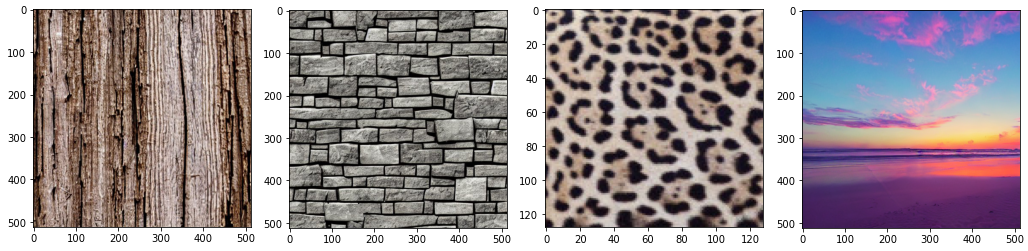
\includegraphics[width=\linewidth]{files/assets/texture.png}
	\caption{As três primeiras imagens são texturas por apresentarem
	um padrão visual estacionário. A quarta imagem apresenta
    uma estrutura não estacionária, não permitindo uma extrapolação
	infinita.}
	\label{img:preview}
\end{figure}

% Mostrar imagens de texturas

 

\section{O que é síntese de textura}

% Processo de gerar uma textura "nova"
% com mesma informação perceptual

O processo de síntese de textura baseado
em amostra não tem uma definição clara
matematicamente, é algo mais intrínseco
à percepção humana. O objetivo é,
a partir de uma amostra de textura,
gerar outras texturas de tamanho
arbitrário que imitam o processo
gerador da amostra. Esse processo
gerador é baseado em métricas
perceptuais, que não podem ser
definidas de forma fechada, pois
podem depender de aspectos
finos da imagem, como forma e 
iluminação.
Assim, os trabalhos na área
nos últimos anos consistem em
tentar descobrir melhores aproximações
para essa métrica perceptual.

% Inserir imagens de exemplo
\begin{figure}[!ht]
	\centering
	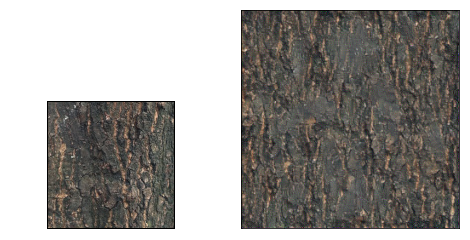
\includegraphics[width=\linewidth*2/3]{files/assets/sinth.png}
	\caption{Exemplo de síntese de textura. A imagem
	maior é visualmente semelhante à imagem menor.}
	\label{img:preview}
\end{figure}


% Pode ser interpretado como uma
% reamostragem da distribuição das texturas

Ao restringir o conjunto de imagens aos
Campos Markovianos, o processo de síntese
pode ser descrito como uma re-amostragem
da distribuição condicional da amostra.
Com isso, o desafio do método passa a ser 
descobrir a distribuição a partir
da amostra.


\chapter{Modelos}

Com o crescimento da área de processamento
de imagens e do poder computacional,
os modelos de Síntese de Textura foram
se aprimorando ao longo do tempo.
As melhorias são tanto de qualidade
do resultado quanto no tempo de 
execução do método. Neste capítulo
será apresentado um breve resumo de
alguns dos principais modelos
da área.



\section{Modelos paramétricos}

Os modelos que fazem a síntese a partir
de um conjunto de estatísticas da amostra
original são chamados modelos paramétricos.
Esses modelos partem de um ruído e fazem
a síntese reduzindo
a diferença entre as estatísticas desse
ruído e da amostra utilizando uma função de 
otimização.
A qualidade do modelo vai depender do
conjunto de estatísticas escolhido
e do tipo de otimização utilizado.

% Heeger and Bergen [6] (matching histograms)

Heegen e Bergen \cite{Heeger1995} foram
um dos pioneiros no ramo. O método
parte de um ruído branco e faz a síntese
aproximando os histogramas das funções
de distribuição acumulada.
O método usa transformações
por pirâmides, que decompõe a imagem
em representações em diferentes escalas,
e faz a aproximação do histograma
em cada uma dessas camadas.
%Eles apresentam
%dois tipos de pirâmides, a Pirâmide 
%Laplaciana, que 
%e a Pirâmide Transladável (Steerable Pyramid)

\begin{figure}[!ht]
	\centering
	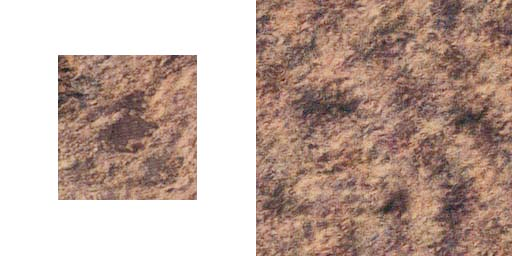
\includegraphics[width=\linewidth*2/3]{files/assets/articles/bergen.png}
	\caption{Síntese de Textura de Heegen e Bergen. O modelo
	conseguia sintetizar elementos estocásticos da textura.}
	\label{img:preview}
\end{figure}

% De Bonet [1] (multi-resolution)

De Bonet \cite{Bonet1997} propôs
um método que calcula a distribuição
conjunta da amostra em diferentes
escalas. Em seguida a amostragem
é feita partindo de escalas mais
grosseiras até escalas mais finas.

\begin{figure}[!ht]
	
\includegraphics[width=\linewidth]{files/assets/articles/bonet2.png}
	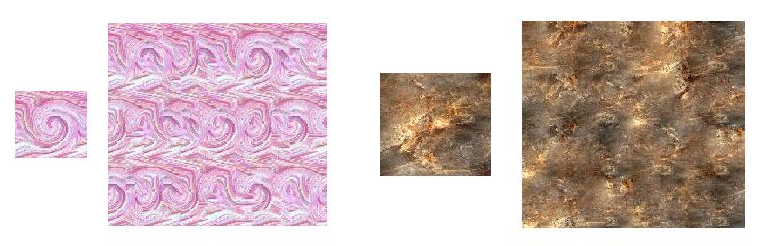
\includegraphics[width=\linewidth]{files/assets/articles/bonet.png}
	\caption{Modelo de De Bonet. O trabalho era feito escala
	por escala. Isso permitia sintetizar elementos mais regulares
    da textura.}
	\label{img:preview}
\end{figure}

% Zhu et al [12] (MRF - Gibbs sampling)
Zhu, Wu e Mumford \cite{Zhu1998}
utiliza um banco de filtros para
obter uma representação da imagem
e extrair o histograma.
Em seguida deriva-se a distribuição
desses filtros para serem re-amostrados
usando a técnica de Gibbs Sampling.

\begin{figure}[!ht]
	\centering
	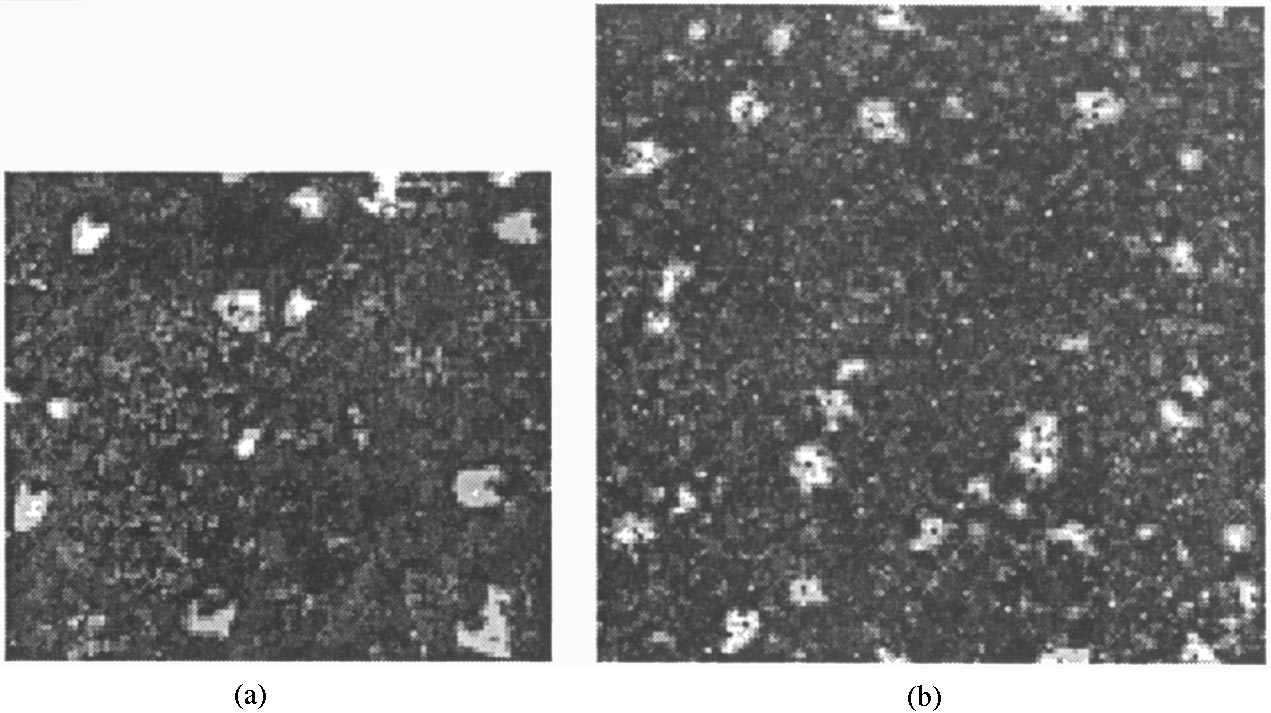
\includegraphics[width=\linewidth*2/3]{files/assets/articles/zhu.png}
	\caption{Modelo de Zhu, Wu e Mumford usando 5 filtros.}
	\label{img:preview}
\end{figure}


% Simoncelli and Portilla [9, 11] (wavelets)

Portilla e Simoncelli \cite{Portilla1999}
propuseram fazer a amostragem usando
as autocorrelações da Transformada
de Wavelet da amostra.

\begin{figure}[!ht]
	\centering
	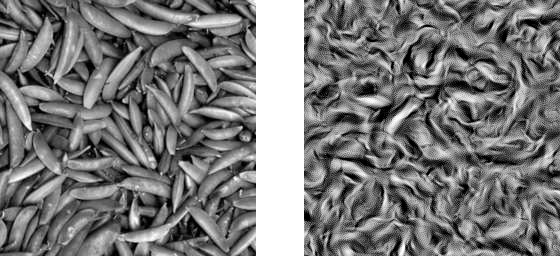
\includegraphics[width=\linewidth*2/3]{files/assets/articles/portilla.png}
	\caption{Teste do modelo de Portilla e Simoncelli com uma
	textura mais estruturado. É possível notar que há uma
	dificuldade em representar tais estruturas.}
	\label{img:preview}
\end{figure}


% Julesz’ hypothesis
% two images are perceptually equivalent if and 
% only if they agree on a set of statistic measurements.

% Falar da dificuldade em definir uma 
% estatística da informao perceptual

Béla Julesz foi um neurocientista que
trabalhava na percepção visual humana.
Em uma de suas publicações \cite{Julesz1981},
Julesz fez experimentos que mostravam
que um conjunto de imagens com mesma
informação visual podem ser representadas
pela densidade do que ele chama de
``Textons'', que são estruturas
como cor e arestas presentes na imagem.
Esse tipo de representação, embora tenha
guiado o trabalho de modelos paramétricos,
não deixa claro como fazer essa representação
em Textons. Assim, na tentativa de encontrar
tal representação, os métodos acabam sendo
difíceis de implementar, e nem sempre
conseguem ter sucesso em diferentes texturas.





\section{Modelos não paramétricos}

% Falar dos modelos que extraem informação
% diretamente da imagem

Diferentemente dos modelos paramétricos,
os modelos não paramétricos não dependem
do cálculo de alguma
estatística da amostra original para
o processo de síntese. Ele gera a imagem
pegando informação diretamente da
amostra de modo a simular a amostragem
da textura.

Essa forma de amostragem foi proposta
inicialmente por Efros e Leung \cite{Efros1999}.
Ela consistia em re-amostrar a textura
pixel por pixel, pegando diretamente
da imagem original o pixel que tem
a vizinhança mais parecida com a vizinhança
de seu destino. Os resultados na época
foram bem superiores aos que se podiam
obter com os métodos paramétricos,
mas a procura por todas as vizinhanças
na amostra tornava o método lento.

\begin{figure}[!ht]
	\centering
	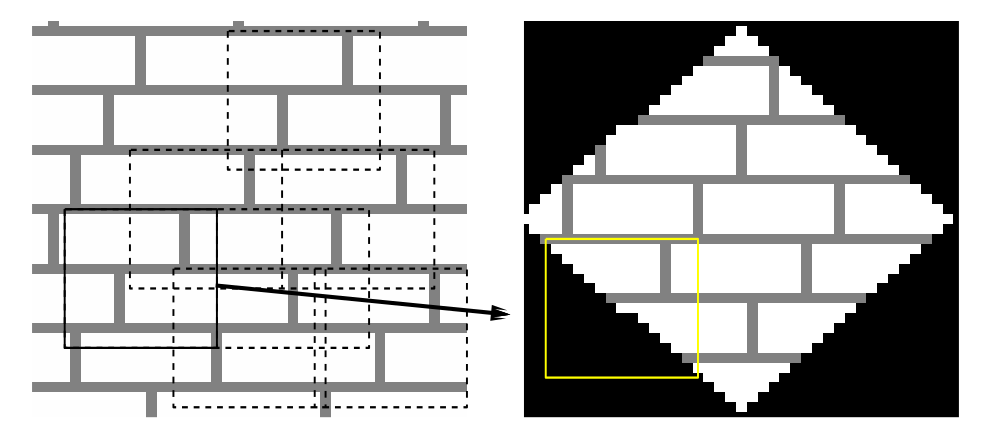
\includegraphics[width=\linewidth*2/3]{files/assets/articles/efros3.png}
	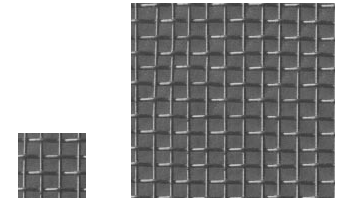
\includegraphics[width=\linewidth*5/6]{files/assets/articles/efros1.png}
	\caption{O algorítmo de Efros e Leung vai escolher o pixel
	com vizinhança mais parecida na amostra.}
	\label{img:preview}
\end{figure}

Mais tarde, Efros e Freeman \cite{Efros2001}
propuseram o método de Quilting (costura),
que fazia a amostragem a partir
de pedaços da imagem original. 
O método consistia em selecionar
janelas de tamanho fixo da amostra
e distribuí-las com uma sobreposição
sobre elas. Em seguida é usado
um algoritmo de min-cut para dividir
essas janelas em pedaços que se encaixam
para formar a nova textura.
Essa abordagem era mais rápida 
computacionalmente do que o método
anterior, e produzia resultados
tão bons quanto.

\begin{figure}[!ht]
	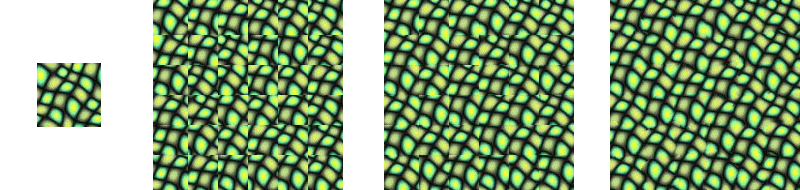
\includegraphics[width=\linewidth]{files/assets/articles/efros2.png}
	\caption{O modelo Quilting de Efros e Freeman escolhe pedaços
	aleatórios da amostra e encaixa os quadrados.}
	\label{img:preview}
\end{figure}

Com os avanços na área,
Vivek Kwatra \cite{Kwatra2005} propôs
uma amostragem fazendo a minimização
do que ele define como função de energia. 
Essa função é a diferença quadrática
entre as vizinhanças da textura gerada
e as vizinhanças mais próximas de cada uma.
O método usa uma variação do algoritmo EM, 
onde na faze ``E'' a energia é diminuída
por mínimos quadrados, e na faze ``M'' a
energia é diminuída escolhendo as
vizinhanças mais próximas na amostra.

\begin{figure}[!ht]
	\centering
	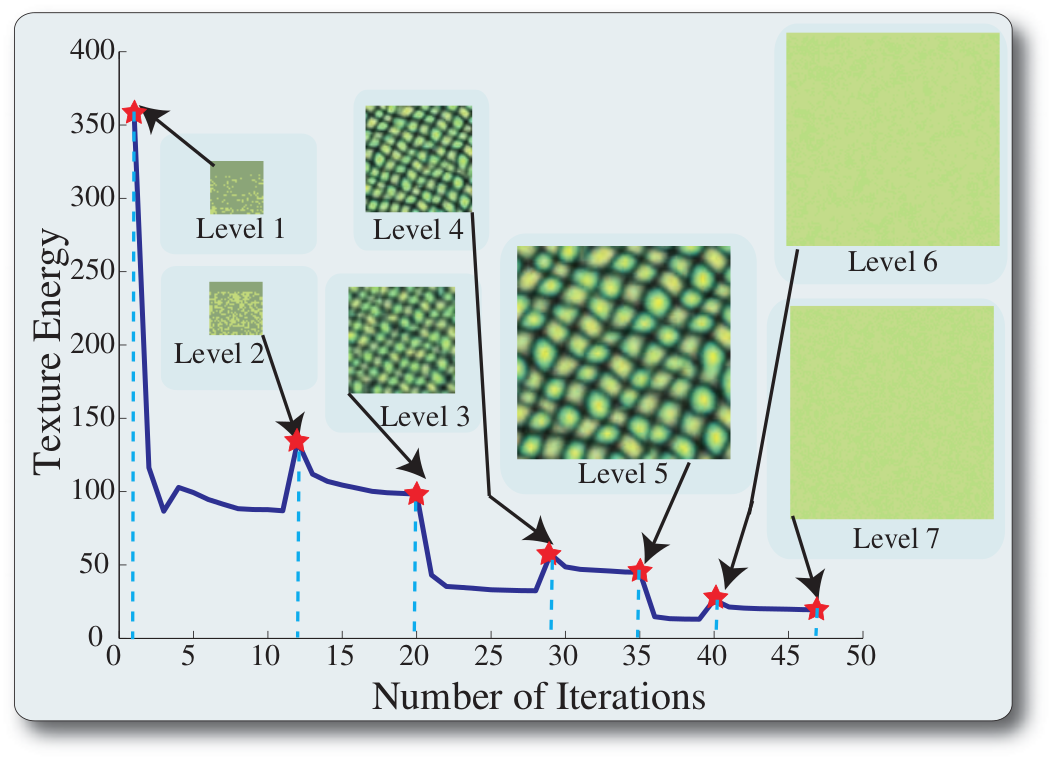
\includegraphics[width=\linewidth*2/3]{files/assets/articles/kwatra.png}
	\caption{Modelo de Vivek Kwatra. A função de energia 
	cai a cada nível de resolução.}
	\label{img:preview}
\end{figure}


\newpage
\section{Modelos de aprendizado profundo}

Os modelos de aprendizado profundo se aproveitam
dos avanços recentes na área de Aprendizagem
de Máquina para melhorar o processo de síntese.
Os métodos a seguir utilizam as representações
geradas por redes treinadas para a detecção
de objetos para melhorar métodos paramétricos
de síntese já existentes.
As representações geradas por essas
redes conseguem sintetizar bem a informação
visual da imagem, oferecendo uma boa
métrica perceptual.

% Gatys

O primeiro a propor Síntese
de Textura baseado nesses modelos foram
Gatys, Ecker e Bethge \cite{Gatys2015}.
O trabalho utiliza as autocorrelações
da textura semelhante ao que foi proposto
por Portilla e Simoncelli, porém, em
vez de utilizar transformações da amostra
escolhidas a mão, utilizam a saída da
rede convolucional pré-treinada. 
Esse método será tratado com detalhes
nesse trabalho, seguindo de uma implementação.

\begin{figure}[!ht]
	\centering
	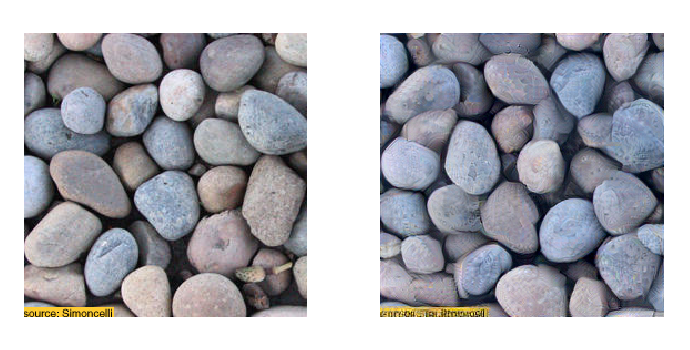
\includegraphics[width=\linewidth*2/3]{files/assets/articles/gatys1.png}
	\caption{Modelo de Gatys, Ecker e Bethge que
	utiliza as matrizes de Gram das convoluções.
	O método não fica muito preso na amostra
	e produz resultados mais criativos.}
	\label{img:preview}
\end{figure}

% Lu

Lu, Zhu e Wu \cite{Lu2016}
utilizam as representações
das redes convolucionais
no lugar do banco de filtros
no método de Zhu, Wu e Mumford,
produzindo melhores resultados sem
se preocupar com o tipo de filtros
escolhidos.

\begin{figure}[!ht]
	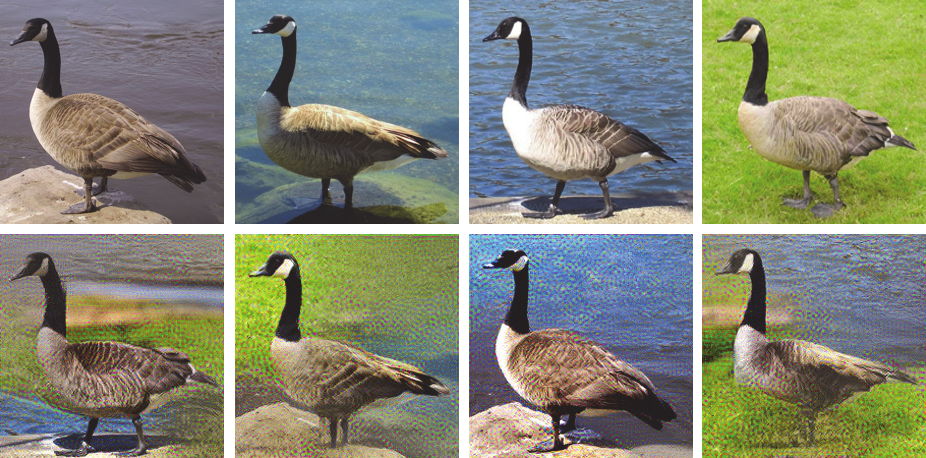
\includegraphics[width=\linewidth]{files/assets/articles/lu.png}
	\caption{Modelo de Lu, Zhu e Wu que pega quatro imagens como
	entrada (as de cima) e gera quatro imagens de saída (as de baixo).}
	\label{img:preview}
\end{figure}


% Falar de multiresolução? (De Bonet)



% ----------------------------------------------------------
% Finaliza a parte no bookmark do PDF
% para que se inicie o bookmark na raiz
% e adiciona espaço de parte no Sumário
% ----------------------------------------------------------
\phantompart

\chapter{Deep Leaning}

% Fazer um resumo

Um dos clássicos problemas na área
de classificação de imagens era o
reconhecimento de dígitos
escritos à mão. 
A dificuldade nesse tipo de problema
vinha pela grande variação de forma
e posição dos números, tornando 
os modelos muito complexos e pouco
precisos. O desenvolvimento
recente na área de Machine Learning
permitiu a criação de modelos
simples capazes de aprender com
os dados e fazer generalizações
precisas, em alguns casos
superando a percepção humana.

Neste capítulo serão apresentadas
técnicas que usam Redes Neurais,
como elas foram desenvolvendo
ao longo dos anos, e como podemos
aplicá-las na Síntese de Textura.


%\cite{Li2021}

\section{Aprendizado de Representação}
%19h


% Hierarquia de representações
No processo de análise de imagens,
precisamos criar representações
que melhor explicam seu conteúdo.
Essas representações podem ser organizadas
hierarquicamente, onde
a primeira identifica
arestas, a segunda indica cantos, etc.
Ao descer no nível das representações
queremos ter uma melhor informação
semântica da imagem.


Para um problema de classificação de imagens,
é preciso saber quais informações são 
úteis para obter uma melhor 
representação de seu conteúdo. 
Uma representação boa esconde informações
redundantes e realçar fatores que 
melhor explicam a imagem.
Bengio, Courville e Vincent
\cite{Bengio2014} falam do importante
papel que a aprendizagem
de representações tem em Machine Learning.
Um algoritmo que aprendesse tais representações
eliminaria o trabalho de desenvolvê-las,
o que tornaria mais rápido a criação de aplicações.


\section{Redes neurais}
%20h

% Definir o que é uma rede neural


Redes Neurais são um tipo 
de modelo de Machine Learning inspirado
em redes de neurônios naturais e como
eles se comunicam. Elas podem ser
representadas por um grafo, onde
cada nó representa um valor e cada aresta
representa uma dependência. Essas
redes podem ter vários formatos
dependendo do tipo de aplicação.

Um exemplo comum de Rede Neural é o Multi Layer
Perceptron. Nesse modelo, a rede é dividida
em camadas de diferentes tamanhos, e o dado
flui da camada de entrada até a saída,
que pode representar uma classificação
da entrada ou uma função geral.

% Imagem MLP

\begin{figure}[!ht]
	\centering
	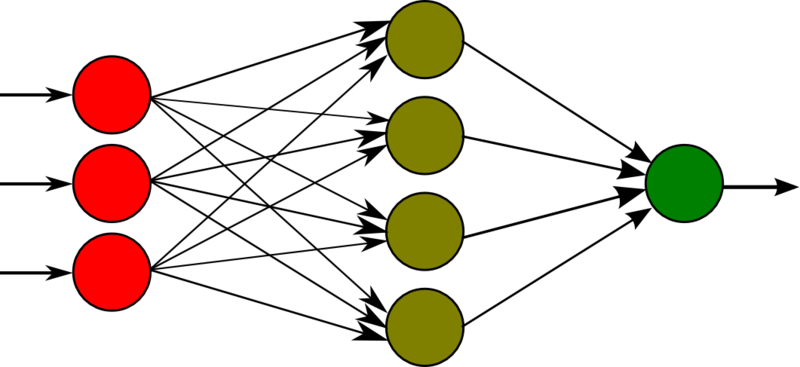
\includegraphics[width=\linewidth*2/3]{files/assets/deeplearning/mlp.png}
	\caption{Rede Multi Layer Perceptron. Cada camada da
	rede atua como uma representação do dado de entrada, que
	é usada para calcular a próxima camada.}
	\label{img:preview}
\end{figure}


Cada camada da rede tem como parâmetros os offsets 
$\mathbf{b}_m$ e uma matriz de pesos $\mathbf{W}_{m\times n}$.
Assim, a transformação da entrada $\mathbf{x}_n$ na saída
$\mathbf{y}_m$ pode ser representada com a seguinte operação:
\begin{equation}
	\mathbf{y} = 
	\varphi\left( \mathbf{W}\mathbf{x} + \mathbf{b} \right),
\end{equation}
onde $\varphi$ é uma função não linear, comummente chamada
de ``função de ativação''. A função não linear
mais comummente usada é a ReLU, que trunca valores
negativos no $0$.

\begin{figure}[!ht]
	\centering
	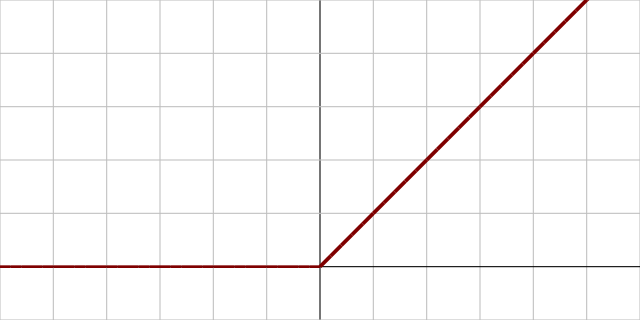
\includegraphics[width=\linewidth*2/3]{files/assets/deeplearning/relu.png}
	\caption{Função ReLU. O seu bico não diferenciável
	facilita a distorcer o espaço de entrada.}
	\label{img:preview}
\end{figure}

%Os parâmetros são tais que minimizam o erro 
%da saída. Essa minimização pode ser feita
%calculando o gradiente 
%\begin{equation}
%	\mathbf{y'} = 
%	\mathbf{W}\varphi'\left( \mathbf{W}\mathbf{x} + \mathbf{b} \right),
%\end{equation}

Os parâmetros são calculados minimizando
uma função de erro na saída. Essa minimização
é feita usando o gradiente dos parâmetros
em relação à função de perda. Como a derivada
de todas as funções aplicadas é conhecida,
o gradiente pode ser calculado computacionalmente
utilizando ``backpropagation''.

%A ideia é ter um modelo
%simples porém bem flexível
%e capaz adaptar ao problema.

% Aproximado universal para qualquer função
% Capacidade de extrapolação

% Dividir qualquer variedade

Esse modelo é útil por envolver operações
bem simples e rápidas de serem calculadas
computacionalmente. Cada camada distorce
o espaço de entrada para torná-lo linearmente
separável no final. Pela sua flexibilidade,
o modelo geralmente é chamado de aproximador 
universal de qualquer função, pois
é capacidade de aprender funções complexas
a partir de amostras.


% Falar do MNIST
...

\section{Redes convolucionais}
%21h

% Aproveitam a informação espacial
% da imagem

% Reduz a quantidade de parâmetros
% Invariante por translação

O Multi Layer Perceptron,
quando aplicado diretamente
nos pixels de uma imagem aparecem
dois problemas consideráveis:
a quantidade de parâmetros cresce muito,
e informações espaciais da imagem
são perdidas. Geralmente um objeto
que queremos identificar pode aparecer
em diferentes posições da imagem,
e ao transformá-la em um vetor,
perdemos essa invariância por translação.
Com base nisso se tornou necessário
desenvolver uma rede que aproveite
a informação espacial da imagem
e que tenha poucos parâmetros.

% Sobre convolução

%A operação de convolução

...



% Sobre CNN (pooling, ReLU)


% Falar das principais arquiteturas (VGG19)

% Revolução na classificação




%\section{Features}

% Mostrar o feature inversion
% e o deep dream 



\section{Síntese de textura com Redes Convolucionais}
%22h

...
% Falar das matrizes de Gram

% Uma boa estatística perceptual

% Falar do L-BFGS 
% (avalia o resultado da função várias vezes
% antes de fazer o passo, é mais eficiente
% em problemas com grande quantidade de parâmetros)

% Falar do padding e do avgpool


% Mostrar os resultados do Gatys

%\section{} %MSLG+Gatys

\iffalse
\chapter{Variações}

O trabalho de síntese de textura
não fica limitado apenas a re-amostrar
a imagem de entrada. Ao longo
dos anos foram aparecendo trabalhos
que aproveitavam os algoritmos
desenvolvidos até então para
criar aplicações como ``inpainting''
e ``renderizações não foto-realísticas''.

...
% Falar de aplicações diferendes de síntese de
% textura

\section{Analogias de Texturas}

% Definir e mostrar resultados
\cite{Hertzmann2001}

...

\begin{figure}[!ht]
	\centering
	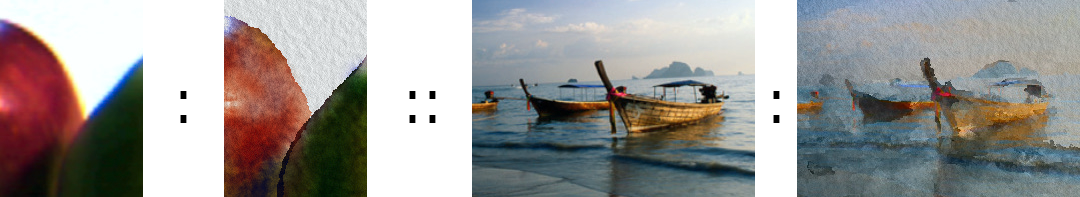
\includegraphics[width=\linewidth*2/3]{files/assets/articles/heartzmann1.png}
	\caption{...}
	\label{img:preview}
\end{figure}

\begin{figure}[!ht]
	\centering
	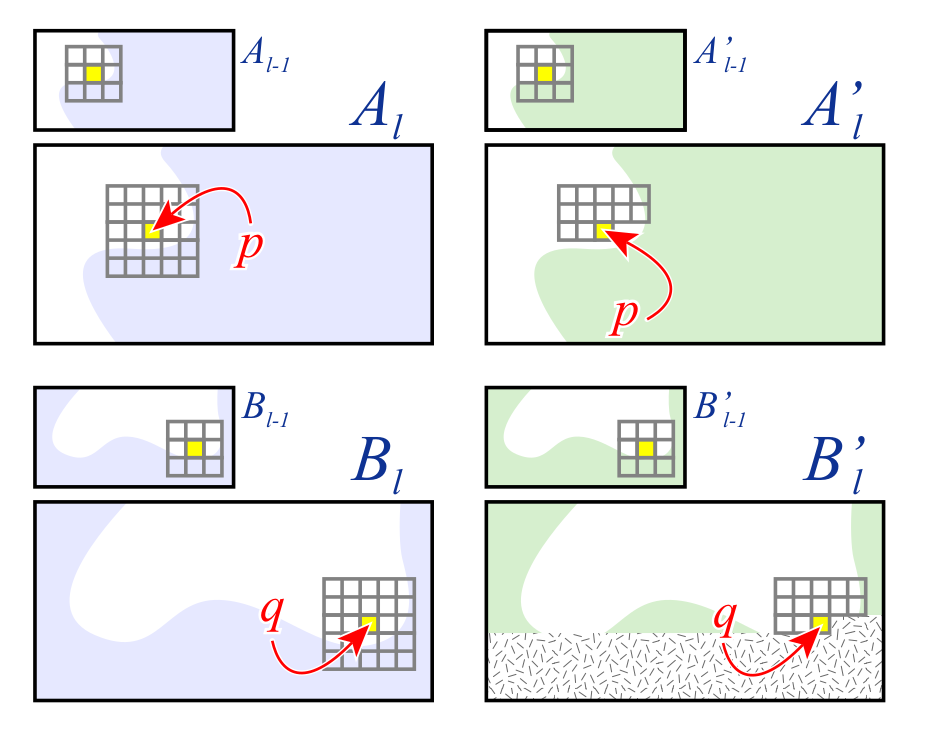
\includegraphics[width=\linewidth*2/3]{files/assets/articles/heartzmann2.png}
	\caption{...}
	\label{img:preview}
\end{figure}


\section{Transferência de estilo} 

O método de ``Style Transfer'' proposto
por Gatys, Ecker e Bethge \cite{Gatys2016}
nos permite, alem de re-amostrar a textura,
controlar a geometria do resultado.
Para isso o algoritmo recebe duas imagens,
uma definirá o estilo
e outra definirá o conteúdo do resultado.

...

\begin{figure}[!ht]
	\centering
	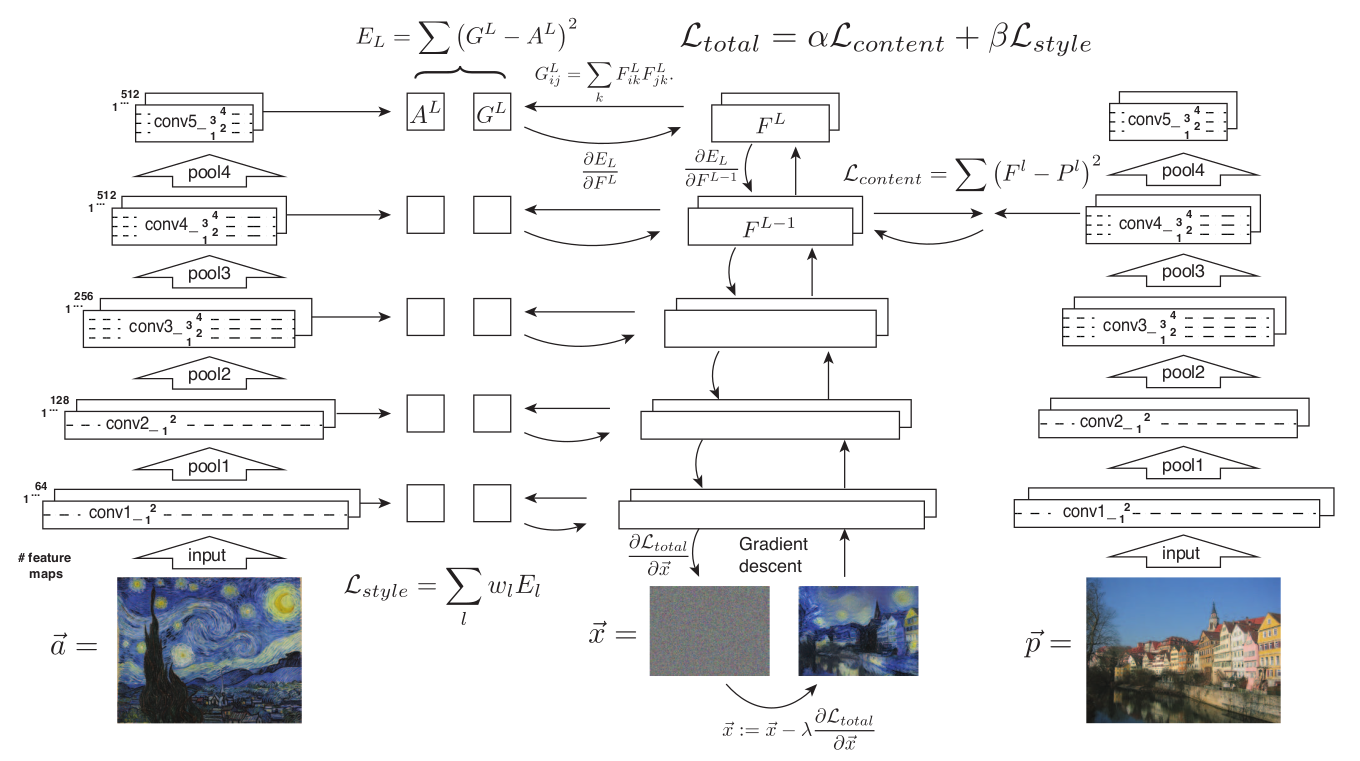
\includegraphics[width=\linewidth]{files/assets/articles/gatys3.png}
	\caption{...}
	\label{img:preview}
\end{figure}


% Definir e mostrar resultados

% Falar do deepart.io?

\fi

\chapter{Resultados}

% Falar da implementação (PyTorch)

Foi feita a implementação do
método de Síntese de Textura
usando a abordagem das matrizes
de Gram. 
Para isso foi utilizada 
a linguagem Python com a
biblioteca PyTorch.
O PyTorch reúne uma série de
funções que facilitaram
a implementação do método.
As principais foram: implementação
nativa da rede VGG-19, operações
aritméticas aceleradas na GPU,
cálculo automático de gradiente,
e implementação de métodos de
otimização.

% Escolha de textura

A primeira ideia era escolher um
conjunto de textura de resolução
$128 \times 128$ e tentar gerar
imagens de $256 \times 256$ pixels.
Foram escolhidos um conjunto de
diferentes tipos de texturas 
para explorar o comportamento
do algoritmo:


% Mostrar os resultados

% Falar do padding e do avgpool

% Textura em movimento

% Style transfer

% Não fica restrito a textura

% Multiescala?

\chapter{Conclusão}


% A principal vantagem de
% Redes neurais é aprender
% métricas perceptuais

% Redes neurais pre-treinadas
% não são apenas para classificação

% PyTorch é uma boa ferramenta
% de deep learning, GPU acelera


%\section{Perspectivas}
% Definir depois

% -----------------------------------
% ELEMENTOS PÓS-TEXTUAIS
% -----------------------------------
\postextual
% ----------------------------------

%\bibliography{biblio}
\printbibliography

%\glossary

% ----------------------------------------------------------
% Apêndices
% ----------------------------------------------------------

% ---
% Inicia os apêndices
% ---
% \begin{apendicesenv}

% % Imprime uma página indicando o início dos apêndices
% \partapendices

% \end{apendicesenv}
% ---

% ----------------------------------------------------------
% Anexos
% ----------------------------------------------------------

% \begin{anexosenv}

% \partanexos

% \end{anexosenv}
"
%---------------------------------------------------------------------
% ÍNDICE REMISSIVO
%---------------------------------------------------------------------
\phantompart
\printindex

\end{document}